% !TEX root = recipeUnderstanding.tex

\section{Introduction}
\vskip -.05in
Human communication takes many forms, including language and vision. For instance, explaining ``how-to'' perform a certain task can be communicated via language (\eg, Do-It-Yourself books) as well as visual (\eg, instructional YouTube videos) information. Regardless of the form, such human-generated communication is generally structured and has a clear beginning, end, and a set of steps in between. Parsing such communication into its semantic steps is the key to understand human activities.

%% AMIR: paragraph Could be removed
Language and vision provide different, but correlating and complementary information. Challenge lies in that both video frames and language (from subtitles generated via Automatic Speech Recognition) are only a noisy, partial observation of the actions being performed. However, the complementary nature of language and vision gives the opportunity to understand the activities only from these partial observations. In this paper, we present a unified model, considering both of the modalities, in order to parse human activities into activity steps with no form of supervision other than requiring videos to be the same category (\eg, all cooking eggs, changing tires, etc.).

%

%requires us to model them jointly. We present a unified model, learnt in a fully unsupervised manner, in order to jointly use these two modalities.

% Furthermore they are
% We utilize these two modalities (video frames and imperfect automatically generated subtitles) in a unified manner in our framework;
% We qualitatively and quantitatively argue that a joint inference is crucial for a successful semantic parsing, particularly when no supervision is employed.


%  the proposed approach on instructional videos from YouTube (\eg, ``Making panckage'', ``How to tie a bow tie'') as they typically have clear steps and provide concrete grounds for demonstrating a semantically meaningful parsing. These videos are often long and manifest a high intra-class variability yet the underlying steps remains well-defined and structured, similar to almost all human communications.

\begin{figure}[h!]
  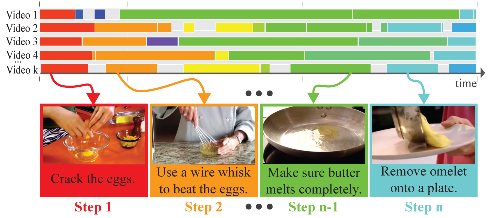
\includegraphics[width=0.48\textwidth]{Figure_1_flattened}
  \vskip -.1in
  \caption{Given a large video collection (frames and subtitles) of an instructional category (\eg, How to cook an omelette?), we discover activity steps (\eg, crack the eggs). We also parse the videos based on the discovered steps.}
  \label{teaser}
  \vspace{-4mm}
\end{figure}


The key idea in our approach is the observation that the large collection of videos, pertaining to the same activity class, typically include only a few objective activity steps, and the variability is the result of exponentially many ways of generating videos from activity steps through subset selection and time ordering. We study this construction based on the large-scale information available in YouTube in the form of instructional videos  (\eg, ``Making pancake'', ``How to tie a bow tie''). Instructional videos have many desirable properties like the volume of the information (\eg, YouTube has 281.000 videos for \emph{"How to tie a bow tie"}) and a well defined notion of activity step.  However, the proposed parsing method is applicable to any type of videos as long as they are composed of a set of steps.

The output of our method can be seen as the semantic ``storyline'' of a rather long and complex video collection (see Fig.~\ref{teaser}). This storyline provides what particular steps are taking place in the video collection, when they are occurring, and what their meaning is (\emph{what-when-how}). This method also puts videos performing the same overall task in common ground and capture their high-level relations.

In the proposed approach, given a collection of videos, we first generate a set of language and visual atoms. These atoms are the result of relating object proposals from each frame as well as detecting the frequent words from subtitles. We then employ a generative \emph{beta process mixture model}, which identifies the activity steps shared among the videos of the same category based on a representation using learned atoms. Although we do not explicity enforce this steps to be semantically meaningful, our results highly correlate with the semantic steps. In our method, we do neither use any spatial or temporal label on actions/steps nor any labels on object categories. We later learn a Markov language model to provide a textual description of the activity steps based on the language atoms it frequently uses.

%This work is the first to discover activity steps for a complex video collection with no supervision over activity steps and/or objects. We are also the first to approach this problem in a multimodal (joint language and vision) manner.
%In addition, our method is capable of providing a caption describing the steps; our approach to captioning is fundamentally different from the existing video/image-to-text work in two aspects: 1) the captions are generated without any supervised caption-clip pairs, 2) our captions are \emph{descriptions} of the semantic steps, yet they are inferred from \emph{narrations}. This is different from the existing captioning work as their reference data is descriptive of the visual information, while the narration over videos often provides complementary information to the visuals and is not necessarily descriptive.
